\documentclass[twoside]{book}

% Packages required by doxygen
\usepackage{fixltx2e}
\usepackage{calc}
\usepackage{doxygen}
\usepackage[export]{adjustbox} % also loads graphicx
\usepackage{graphicx}
\usepackage[utf8]{inputenc}
\usepackage{makeidx}
\usepackage{multicol}
\usepackage{multirow}
\PassOptionsToPackage{warn}{textcomp}
\usepackage{textcomp}
\usepackage[nointegrals]{wasysym}
\usepackage[table]{xcolor}

% Font selection
\usepackage[T1]{fontenc}
\usepackage[scaled=.90]{helvet}
\usepackage{courier}
\usepackage{amssymb}
\usepackage{sectsty}
\renewcommand{\familydefault}{\sfdefault}
\allsectionsfont{%
  \fontseries{bc}\selectfont%
  \color{darkgray}%
}
\renewcommand{\DoxyLabelFont}{%
  \fontseries{bc}\selectfont%
  \color{darkgray}%
}
\newcommand{\+}{\discretionary{\mbox{\scriptsize$\hookleftarrow$}}{}{}}

% Page & text layout
\usepackage{geometry}
\geometry{%
  a4paper,%
  top=2.5cm,%
  bottom=2.5cm,%
  left=2.5cm,%
  right=2.5cm%
}
\tolerance=750
\hfuzz=15pt
\hbadness=750
\setlength{\emergencystretch}{15pt}
\setlength{\parindent}{0cm}
\setlength{\parskip}{3ex plus 2ex minus 2ex}
\makeatletter
\renewcommand{\paragraph}{%
  \@startsection{paragraph}{4}{0ex}{-1.0ex}{1.0ex}{%
    \normalfont\normalsize\bfseries\SS@parafont%
  }%
}
\renewcommand{\subparagraph}{%
  \@startsection{subparagraph}{5}{0ex}{-1.0ex}{1.0ex}{%
    \normalfont\normalsize\bfseries\SS@subparafont%
  }%
}
\makeatother

% Headers & footers
\usepackage{fancyhdr}
\pagestyle{fancyplain}
\fancyhead[LE]{\fancyplain{}{\bfseries\thepage}}
\fancyhead[CE]{\fancyplain{}{}}
\fancyhead[RE]{\fancyplain{}{\bfseries\leftmark}}
\fancyhead[LO]{\fancyplain{}{\bfseries\rightmark}}
\fancyhead[CO]{\fancyplain{}{}}
\fancyhead[RO]{\fancyplain{}{\bfseries\thepage}}
\fancyfoot[LE]{\fancyplain{}{}}
\fancyfoot[CE]{\fancyplain{}{}}
\fancyfoot[RE]{\fancyplain{}{\bfseries\scriptsize Generated by Doxygen }}
\fancyfoot[LO]{\fancyplain{}{\bfseries\scriptsize Generated by Doxygen }}
\fancyfoot[CO]{\fancyplain{}{}}
\fancyfoot[RO]{\fancyplain{}{}}
\renewcommand{\footrulewidth}{0.4pt}
\renewcommand{\chaptermark}[1]{%
  \markboth{#1}{}%
}
\renewcommand{\sectionmark}[1]{%
  \markright{\thesection\ #1}%
}

% Indices & bibliography
\usepackage{natbib}
\usepackage[titles]{tocloft}
\setcounter{tocdepth}{3}
\setcounter{secnumdepth}{5}
\makeindex

% Hyperlinks (required, but should be loaded last)
\usepackage{ifpdf}
\ifpdf
  \usepackage[pdftex,pagebackref=true]{hyperref}
\else
  \usepackage[ps2pdf,pagebackref=true]{hyperref}
\fi
\hypersetup{%
  colorlinks=true,%
  linkcolor=blue,%
  citecolor=blue,%
  unicode%
}

% Custom commands
\newcommand{\clearemptydoublepage}{%
  \newpage{\pagestyle{empty}\cleardoublepage}%
}

\usepackage{caption}
\captionsetup{labelsep=space,justification=centering,font={bf},singlelinecheck=off,skip=4pt,position=top}

%===== C O N T E N T S =====

\begin{document}

% Titlepage & ToC
\hypersetup{pageanchor=false,
             bookmarksnumbered=true,
             pdfencoding=unicode
            }
\pagenumbering{alph}
\begin{titlepage}
\vspace*{7cm}
\begin{center}%
{\Large Heislab }\\
\vspace*{1cm}
{\large Generated by Doxygen 1.8.13}\\
\end{center}
\end{titlepage}
\clearemptydoublepage
\pagenumbering{roman}
\tableofcontents
\clearemptydoublepage
\pagenumbering{arabic}
\hypersetup{pageanchor=true}

%--- Begin generated contents ---
\chapter{Data Structure Index}
\section{Data Structures}
Here are the data structures with brief descriptions\+:\begin{DoxyCompactList}
\item\contentsline{section}{\hyperlink{structPanel}{Panel} \\*\hyperlink{structPanel}{Panel} struct to contain information about buttons pushed on elevator panels }{\pageref{structPanel}}{}
\item\contentsline{section}{\hyperlink{structState}{State} \\*Clean\+Orders function to clear all orders }{\pageref{structState}}{}
\end{DoxyCompactList}

\chapter{File Index}
\section{File List}
Here is a list of all documented files with brief descriptions\+:\begin{DoxyCompactList}
\item\contentsline{section}{source/\hyperlink{hardware_8h}{hardware.\+h} \\*Driver for the elevator hardware }{\pageref{hardware_8h}}{}
\item\contentsline{section}{source/{\bfseries main.\+c} }{\pageref{main_8c}}{}
\item\contentsline{section}{source/\hyperlink{Motor_8c}{Motor.\+c} \\*Struct and functionality to handle state of elevator }{\pageref{Motor_8c}}{}
\item\contentsline{section}{source/\hyperlink{Motor_8h}{Motor.\+h} \\*Struct and functionality to handle state of elevator }{\pageref{Motor_8h}}{}
\item\contentsline{section}{source/\hyperlink{Panel_8c}{Panel.\+c} \\*Implementation of \hyperlink{Panel_8h}{Panel.\+h} }{\pageref{Panel_8c}}{}
\item\contentsline{section}{source/\hyperlink{Panel_8h}{Panel.\+h} \\*Functionality in conjunction with elevator panels }{\pageref{Panel_8h}}{}
\item\contentsline{section}{source/\hyperlink{State_8c}{State.\+c} \\*Implementation of \hyperlink{State_8h}{State.\+h} }{\pageref{State_8c}}{}
\item\contentsline{section}{source/\hyperlink{State_8h}{State.\+h} \\*Struct and functionality to handle state of elevator }{\pageref{State_8h}}{}
\end{DoxyCompactList}

\chapter{Data Structure Documentation}
\hypertarget{structPanel}{}\section{Panel Struct Reference}
\label{structPanel}\index{Panel@{Panel}}


\hyperlink{structPanel}{Panel} struct to contain information about buttons pushed on elevator panels.  




{\ttfamily \#include $<$Panel.\+h$>$}

\subsection*{Data Fields}
\begin{DoxyCompactItemize}
\item 
\mbox{\Hypertarget{structPanel_a224927d561a376b80541efcbf5c21ff2}\label{structPanel_a224927d561a376b80541efcbf5c21ff2}} 
int {\bfseries orders} \mbox{[}8\mbox{]}
\item 
\mbox{\Hypertarget{structPanel_a07700ed7f0590ce3a679d82665b8406b}\label{structPanel_a07700ed7f0590ce3a679d82665b8406b}} 
bool {\bfseries stop}
\item 
\mbox{\Hypertarget{structPanel_ae08e0701f78804db92e26cecb835f1c5}\label{structPanel_ae08e0701f78804db92e26cecb835f1c5}} 
bool {\bfseries obstruction}
\end{DoxyCompactItemize}


\subsection{Detailed Description}
\hyperlink{structPanel}{Panel} struct to contain information about buttons pushed on elevator panels. 


\begin{DoxyParams}[1]{Parameters}
\mbox{\tt out}  & {\em orders} & Two-\/dimensional array containing information about incoming orders \\
\hline
\mbox{\tt out}  & {\em stop} & Boolean variable to indicate whether stop-\/button is pushed or not \\
\hline
\mbox{\tt out}  & {\em obstruction} & Boolean variable to indicate whether obstruction-\/switch is active or not \\
\hline
\end{DoxyParams}


Definition at line 23 of file Panel.\+h.



The documentation for this struct was generated from the following file\+:\begin{DoxyCompactItemize}
\item 
source/\hyperlink{Panel_8h}{Panel.\+h}\end{DoxyCompactItemize}

\hypertarget{structState}{}\section{State Struct Reference}
\label{structState}\index{State@{State}}


clean\+Orders function to clear all orders  




{\ttfamily \#include $<$State.\+h$>$}

\subsection*{Data Fields}
\begin{DoxyCompactItemize}
\item 
\mbox{\Hypertarget{structState_a9a4974e82bc7b99af7715b3189487a31}\label{structState_a9a4974e82bc7b99af7715b3189487a31}} 
int {\bfseries prev\+Floor}
\item 
\mbox{\Hypertarget{structState_a4cd2ebda127f8b9823eba7c826b10a75}\label{structState_a4cd2ebda127f8b9823eba7c826b10a75}} 
int {\bfseries current\+Floor}
\item 
\mbox{\Hypertarget{structState_a3b31c590da55414522eff4e78446a16a}\label{structState_a3b31c590da55414522eff4e78446a16a}} 
int {\bfseries between\+Floors} \mbox{[}2\mbox{]}
\item 
\mbox{\Hypertarget{structState_a832d2d78380f35e196d9d5852745e443}\label{structState_a832d2d78380f35e196d9d5852745e443}} 
int {\bfseries Direction}
\item 
\mbox{\Hypertarget{structState_a43387fbee52a7c410724b9e11c07de4c}\label{structState_a43387fbee52a7c410724b9e11c07de4c}} 
int {\bfseries prev\+Direction}
\item 
\mbox{\Hypertarget{structState_a6fa44c270fd2f9880649db7c26aec6da}\label{structState_a6fa44c270fd2f9880649db7c26aec6da}} 
int {\bfseries reached\+Floor}
\end{DoxyCompactItemize}


\subsection{Detailed Description}
clean\+Orders function to clear all orders 

Definition at line 21 of file State.\+h.



The documentation for this struct was generated from the following file\+:\begin{DoxyCompactItemize}
\item 
source/\hyperlink{State_8h}{State.\+h}\end{DoxyCompactItemize}

\chapter{File Documentation}
\hypertarget{hardware_8h}{}\section{source/hardware.h File Reference}
\label{hardware_8h}\index{source/hardware.\+h@{source/hardware.\+h}}


Driver for the elevator hardware.  


This graph shows which files directly or indirectly include this file\+:
\nopagebreak
\begin{figure}[H]
\begin{center}
\leavevmode
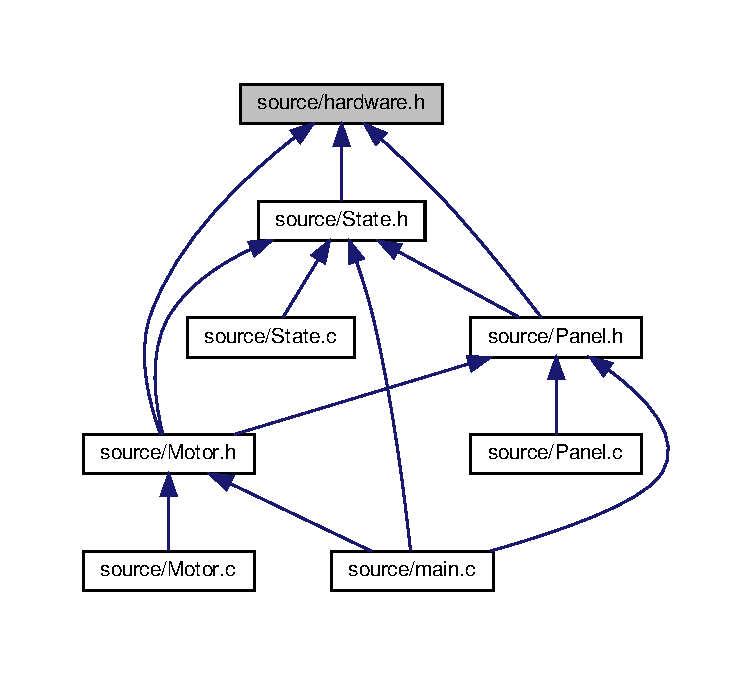
\includegraphics[width=350pt]{hardware_8h__dep__incl}
\end{center}
\end{figure}
\subsection*{Macros}
\begin{DoxyCompactItemize}
\item 
\mbox{\Hypertarget{hardware_8h_ae9e42615eade15633bd8c03b7a271a00}\label{hardware_8h_ae9e42615eade15633bd8c03b7a271a00}} 
\#define {\bfseries H\+A\+R\+D\+W\+A\+R\+E\+\_\+\+N\+U\+M\+B\+E\+R\+\_\+\+O\+F\+\_\+\+F\+L\+O\+O\+RS}~4
\end{DoxyCompactItemize}
\subsection*{Enumerations}
\begin{DoxyCompactItemize}
\item 
\mbox{\Hypertarget{hardware_8h_a2167c399a24df296afc432bcb88228af}\label{hardware_8h_a2167c399a24df296afc432bcb88228af}} 
enum \hyperlink{hardware_8h_a2167c399a24df296afc432bcb88228af}{Hardware\+Movement} \{ {\bfseries H\+A\+R\+D\+W\+A\+R\+E\+\_\+\+M\+O\+V\+E\+M\+E\+N\+T\+\_\+\+UP}, 
{\bfseries H\+A\+R\+D\+W\+A\+R\+E\+\_\+\+M\+O\+V\+E\+M\+E\+N\+T\+\_\+\+S\+T\+OP}, 
{\bfseries H\+A\+R\+D\+W\+A\+R\+E\+\_\+\+M\+O\+V\+E\+M\+E\+N\+T\+\_\+\+D\+O\+WN}
 \}\begin{DoxyCompactList}\small\item\em Movement type used in {\ttfamily hardware\+\_\+command\+\_\+movement}. \end{DoxyCompactList}
\item 
\mbox{\Hypertarget{hardware_8h_a796a8de8ce0ae769d7dbd3327a7bdbe7}\label{hardware_8h_a796a8de8ce0ae769d7dbd3327a7bdbe7}} 
enum \hyperlink{hardware_8h_a796a8de8ce0ae769d7dbd3327a7bdbe7}{Hardware\+Order} \{ {\bfseries H\+A\+R\+D\+W\+A\+R\+E\+\_\+\+O\+R\+D\+E\+R\+\_\+\+UP}, 
{\bfseries H\+A\+R\+D\+W\+A\+R\+E\+\_\+\+O\+R\+D\+E\+R\+\_\+\+I\+N\+S\+I\+DE}, 
{\bfseries H\+A\+R\+D\+W\+A\+R\+E\+\_\+\+O\+R\+D\+E\+R\+\_\+\+D\+O\+WN}
 \}\begin{DoxyCompactList}\small\item\em Order type used in {\ttfamily hardware\+\_\+read\+\_\+order} and in {\ttfamily hardware\+\_\+command\+\_\+order\+\_\+light}. \end{DoxyCompactList}
\end{DoxyCompactItemize}
\subsection*{Functions}
\begin{DoxyCompactItemize}
\item 
int \hyperlink{hardware_8h_a054b8fb8768311d46be58d6a4890d771}{hardware\+\_\+init} ()
\begin{DoxyCompactList}\small\item\em Initializes the elevator control hardware. Must be called once before other calls to the elevator hardware driver. \end{DoxyCompactList}\item 
void \hyperlink{hardware_8h_a01de081ef0510a111053c18cd31afa27}{hardware\+\_\+command\+\_\+movement} (\hyperlink{hardware_8h_a2167c399a24df296afc432bcb88228af}{Hardware\+Movement} movement)
\begin{DoxyCompactList}\small\item\em Commands the elevator to either move up or down, or commands it to halt. \end{DoxyCompactList}\item 
int \hyperlink{hardware_8h_a4a77b27c86675c00b513db3445966804}{hardware\+\_\+read\+\_\+stop\+\_\+signal} ()
\begin{DoxyCompactList}\small\item\em Polls the hardware for the current stop signal. \end{DoxyCompactList}\item 
int \hyperlink{hardware_8h_a459fe57a3ee4bc2a28e8a15b2ab14c2d}{hardware\+\_\+read\+\_\+obstruction\+\_\+signal} ()
\begin{DoxyCompactList}\small\item\em Polls the hardware for the current obstruction signal. \end{DoxyCompactList}\item 
int \hyperlink{hardware_8h_ab048489e6302bb5604aad753f2d7d501}{hardware\+\_\+read\+\_\+floor\+\_\+sensor} (int floor)
\begin{DoxyCompactList}\small\item\em Polls the floor sensor for the given {\ttfamily floor}. \end{DoxyCompactList}\item 
int \hyperlink{hardware_8h_a87917f3aa093fb46ca821a400d011ee8}{hardware\+\_\+read\+\_\+order} (int floor, \hyperlink{hardware_8h_a796a8de8ce0ae769d7dbd3327a7bdbe7}{Hardware\+Order} order\+\_\+type)
\begin{DoxyCompactList}\small\item\em Polls the hardware for the status of orders from floor {\ttfamily floor} of type {\ttfamily order\+\_\+type}. \end{DoxyCompactList}\item 
void \hyperlink{hardware_8h_a80d99ddaa8e7b58c9a88b60ea553c1b6}{hardware\+\_\+command\+\_\+door\+\_\+open} (int door\+\_\+open)
\begin{DoxyCompactList}\small\item\em Commands the hardware to open-\/ or close the elevator door. \end{DoxyCompactList}\item 
void \hyperlink{hardware_8h_a407a6ec035ba357de6aa0fbe55501d1e}{hardware\+\_\+command\+\_\+floor\+\_\+indicator\+\_\+on} (int floor)
\begin{DoxyCompactList}\small\item\em Commands the hardware to turn on the floor indicator for {\ttfamily floor}. All indicators all mutually exclusive; other indicator lights will turn off. \end{DoxyCompactList}\item 
void \hyperlink{hardware_8h_aa75b3ac17f72b25946414f48d0063a10}{hardware\+\_\+command\+\_\+stop\+\_\+light} (int on)
\begin{DoxyCompactList}\small\item\em Sets the light in the panel stop button. \end{DoxyCompactList}\item 
void \hyperlink{hardware_8h_aa9b33faa52f0ec5b614d3e7dc05be140}{hardware\+\_\+command\+\_\+order\+\_\+light} (int floor, \hyperlink{hardware_8h_a796a8de8ce0ae769d7dbd3327a7bdbe7}{Hardware\+Order} order\+\_\+type, int on)
\begin{DoxyCompactList}\small\item\em Sets the light in a button corresponding to an order of type {\ttfamily order\+\_\+type}, at floor {\ttfamily floor}. \end{DoxyCompactList}\end{DoxyCompactItemize}


\subsection{Detailed Description}
Driver for the elevator hardware. 

Neatly wraps up Martin Korsgaard\textquotesingle{}s spaghetti from 2006 ;)

Kolbjørn Austreng 

\subsection{Function Documentation}
\mbox{\Hypertarget{hardware_8h_a80d99ddaa8e7b58c9a88b60ea553c1b6}\label{hardware_8h_a80d99ddaa8e7b58c9a88b60ea553c1b6}} 
\index{hardware.\+h@{hardware.\+h}!hardware\+\_\+command\+\_\+door\+\_\+open@{hardware\+\_\+command\+\_\+door\+\_\+open}}
\index{hardware\+\_\+command\+\_\+door\+\_\+open@{hardware\+\_\+command\+\_\+door\+\_\+open}!hardware.\+h@{hardware.\+h}}
\subsubsection{\texorpdfstring{hardware\+\_\+command\+\_\+door\+\_\+open()}{hardware\_command\_door\_open()}}
{\footnotesize\ttfamily void hardware\+\_\+command\+\_\+door\+\_\+open (\begin{DoxyParamCaption}\item[{int}]{door\+\_\+open }\end{DoxyParamCaption})}



Commands the hardware to open-\/ or close the elevator door. 


\begin{DoxyParams}{Parameters}
{\em door\+\_\+open} & A truthy value (non-\/zero) to open the door; 0 to close. \\
\hline
\end{DoxyParams}
\mbox{\Hypertarget{hardware_8h_a407a6ec035ba357de6aa0fbe55501d1e}\label{hardware_8h_a407a6ec035ba357de6aa0fbe55501d1e}} 
\index{hardware.\+h@{hardware.\+h}!hardware\+\_\+command\+\_\+floor\+\_\+indicator\+\_\+on@{hardware\+\_\+command\+\_\+floor\+\_\+indicator\+\_\+on}}
\index{hardware\+\_\+command\+\_\+floor\+\_\+indicator\+\_\+on@{hardware\+\_\+command\+\_\+floor\+\_\+indicator\+\_\+on}!hardware.\+h@{hardware.\+h}}
\subsubsection{\texorpdfstring{hardware\+\_\+command\+\_\+floor\+\_\+indicator\+\_\+on()}{hardware\_command\_floor\_indicator\_on()}}
{\footnotesize\ttfamily void hardware\+\_\+command\+\_\+floor\+\_\+indicator\+\_\+on (\begin{DoxyParamCaption}\item[{int}]{floor }\end{DoxyParamCaption})}



Commands the hardware to turn on the floor indicator for {\ttfamily floor}. All indicators all mutually exclusive; other indicator lights will turn off. 


\begin{DoxyParams}{Parameters}
{\em floor} & Floor to turn on the indicator for.\\
\hline
\end{DoxyParams}
\begin{DoxyWarning}{Warning}
Owing to peculiarities in the hardware construction, there will always be one indicator active. 
\end{DoxyWarning}
\mbox{\Hypertarget{hardware_8h_a01de081ef0510a111053c18cd31afa27}\label{hardware_8h_a01de081ef0510a111053c18cd31afa27}} 
\index{hardware.\+h@{hardware.\+h}!hardware\+\_\+command\+\_\+movement@{hardware\+\_\+command\+\_\+movement}}
\index{hardware\+\_\+command\+\_\+movement@{hardware\+\_\+command\+\_\+movement}!hardware.\+h@{hardware.\+h}}
\subsubsection{\texorpdfstring{hardware\+\_\+command\+\_\+movement()}{hardware\_command\_movement()}}
{\footnotesize\ttfamily void hardware\+\_\+command\+\_\+movement (\begin{DoxyParamCaption}\item[{\hyperlink{hardware_8h_a2167c399a24df296afc432bcb88228af}{Hardware\+Movement}}]{movement }\end{DoxyParamCaption})}



Commands the elevator to either move up or down, or commands it to halt. 


\begin{DoxyParams}{Parameters}
{\em movement} & Commanded movement. \\
\hline
\end{DoxyParams}
\mbox{\Hypertarget{hardware_8h_aa9b33faa52f0ec5b614d3e7dc05be140}\label{hardware_8h_aa9b33faa52f0ec5b614d3e7dc05be140}} 
\index{hardware.\+h@{hardware.\+h}!hardware\+\_\+command\+\_\+order\+\_\+light@{hardware\+\_\+command\+\_\+order\+\_\+light}}
\index{hardware\+\_\+command\+\_\+order\+\_\+light@{hardware\+\_\+command\+\_\+order\+\_\+light}!hardware.\+h@{hardware.\+h}}
\subsubsection{\texorpdfstring{hardware\+\_\+command\+\_\+order\+\_\+light()}{hardware\_command\_order\_light()}}
{\footnotesize\ttfamily void hardware\+\_\+command\+\_\+order\+\_\+light (\begin{DoxyParamCaption}\item[{int}]{floor,  }\item[{\hyperlink{hardware_8h_a796a8de8ce0ae769d7dbd3327a7bdbe7}{Hardware\+Order}}]{order\+\_\+type,  }\item[{int}]{on }\end{DoxyParamCaption})}



Sets the light in a button corresponding to an order of type {\ttfamily order\+\_\+type}, at floor {\ttfamily floor}. 


\begin{DoxyParams}{Parameters}
{\em floor} & The floor of the order indicator. \\
\hline
{\em order\+\_\+type} & The type of order. \\
\hline
{\em on} & A truthy value (non-\/zero) to turn the light on; 0 to turn it off. \\
\hline
\end{DoxyParams}
\mbox{\Hypertarget{hardware_8h_aa75b3ac17f72b25946414f48d0063a10}\label{hardware_8h_aa75b3ac17f72b25946414f48d0063a10}} 
\index{hardware.\+h@{hardware.\+h}!hardware\+\_\+command\+\_\+stop\+\_\+light@{hardware\+\_\+command\+\_\+stop\+\_\+light}}
\index{hardware\+\_\+command\+\_\+stop\+\_\+light@{hardware\+\_\+command\+\_\+stop\+\_\+light}!hardware.\+h@{hardware.\+h}}
\subsubsection{\texorpdfstring{hardware\+\_\+command\+\_\+stop\+\_\+light()}{hardware\_command\_stop\_light()}}
{\footnotesize\ttfamily void hardware\+\_\+command\+\_\+stop\+\_\+light (\begin{DoxyParamCaption}\item[{int}]{on }\end{DoxyParamCaption})}



Sets the light in the panel stop button. 


\begin{DoxyParams}{Parameters}
{\em on} & A truthy value (non-\/zero) to turn the light on; 0 to turn it off. \\
\hline
\end{DoxyParams}
\mbox{\Hypertarget{hardware_8h_a054b8fb8768311d46be58d6a4890d771}\label{hardware_8h_a054b8fb8768311d46be58d6a4890d771}} 
\index{hardware.\+h@{hardware.\+h}!hardware\+\_\+init@{hardware\+\_\+init}}
\index{hardware\+\_\+init@{hardware\+\_\+init}!hardware.\+h@{hardware.\+h}}
\subsubsection{\texorpdfstring{hardware\+\_\+init()}{hardware\_init()}}
{\footnotesize\ttfamily int hardware\+\_\+init (\begin{DoxyParamCaption}{ }\end{DoxyParamCaption})}



Initializes the elevator control hardware. Must be called once before other calls to the elevator hardware driver. 

\begin{DoxyReturn}{Returns}
0 on success. Non-\/zero for failure. 
\end{DoxyReturn}
\mbox{\Hypertarget{hardware_8h_ab048489e6302bb5604aad753f2d7d501}\label{hardware_8h_ab048489e6302bb5604aad753f2d7d501}} 
\index{hardware.\+h@{hardware.\+h}!hardware\+\_\+read\+\_\+floor\+\_\+sensor@{hardware\+\_\+read\+\_\+floor\+\_\+sensor}}
\index{hardware\+\_\+read\+\_\+floor\+\_\+sensor@{hardware\+\_\+read\+\_\+floor\+\_\+sensor}!hardware.\+h@{hardware.\+h}}
\subsubsection{\texorpdfstring{hardware\+\_\+read\+\_\+floor\+\_\+sensor()}{hardware\_read\_floor\_sensor()}}
{\footnotesize\ttfamily int hardware\+\_\+read\+\_\+floor\+\_\+sensor (\begin{DoxyParamCaption}\item[{int}]{floor }\end{DoxyParamCaption})}



Polls the floor sensor for the given {\ttfamily floor}. 


\begin{DoxyParams}{Parameters}
{\em floor} & Inquired floor.\\
\hline
\end{DoxyParams}
\begin{DoxyReturn}{Returns}
1 if the elevator is at {\ttfamily floor}, otherwise 0; 
\end{DoxyReturn}
\mbox{\Hypertarget{hardware_8h_a459fe57a3ee4bc2a28e8a15b2ab14c2d}\label{hardware_8h_a459fe57a3ee4bc2a28e8a15b2ab14c2d}} 
\index{hardware.\+h@{hardware.\+h}!hardware\+\_\+read\+\_\+obstruction\+\_\+signal@{hardware\+\_\+read\+\_\+obstruction\+\_\+signal}}
\index{hardware\+\_\+read\+\_\+obstruction\+\_\+signal@{hardware\+\_\+read\+\_\+obstruction\+\_\+signal}!hardware.\+h@{hardware.\+h}}
\subsubsection{\texorpdfstring{hardware\+\_\+read\+\_\+obstruction\+\_\+signal()}{hardware\_read\_obstruction\_signal()}}
{\footnotesize\ttfamily int hardware\+\_\+read\+\_\+obstruction\+\_\+signal (\begin{DoxyParamCaption}{ }\end{DoxyParamCaption})}



Polls the hardware for the current obstruction signal. 

\begin{DoxyReturn}{Returns}
1 if the obstruction signal is high; 0 if it is low. 
\end{DoxyReturn}
\mbox{\Hypertarget{hardware_8h_a87917f3aa093fb46ca821a400d011ee8}\label{hardware_8h_a87917f3aa093fb46ca821a400d011ee8}} 
\index{hardware.\+h@{hardware.\+h}!hardware\+\_\+read\+\_\+order@{hardware\+\_\+read\+\_\+order}}
\index{hardware\+\_\+read\+\_\+order@{hardware\+\_\+read\+\_\+order}!hardware.\+h@{hardware.\+h}}
\subsubsection{\texorpdfstring{hardware\+\_\+read\+\_\+order()}{hardware\_read\_order()}}
{\footnotesize\ttfamily int hardware\+\_\+read\+\_\+order (\begin{DoxyParamCaption}\item[{int}]{floor,  }\item[{\hyperlink{hardware_8h_a796a8de8ce0ae769d7dbd3327a7bdbe7}{Hardware\+Order}}]{order\+\_\+type }\end{DoxyParamCaption})}



Polls the hardware for the status of orders from floor {\ttfamily floor} of type {\ttfamily order\+\_\+type}. 


\begin{DoxyParams}{Parameters}
{\em floor} & Inquired floor. \\
\hline
{\em order\+\_\+type} & \\
\hline
\end{DoxyParams}
\begin{DoxyReturn}{Returns}
1 if the combination of {\ttfamily floor} and {\ttfamily order\+\_\+type} is being requested, otherwise 0. 
\end{DoxyReturn}
\mbox{\Hypertarget{hardware_8h_a4a77b27c86675c00b513db3445966804}\label{hardware_8h_a4a77b27c86675c00b513db3445966804}} 
\index{hardware.\+h@{hardware.\+h}!hardware\+\_\+read\+\_\+stop\+\_\+signal@{hardware\+\_\+read\+\_\+stop\+\_\+signal}}
\index{hardware\+\_\+read\+\_\+stop\+\_\+signal@{hardware\+\_\+read\+\_\+stop\+\_\+signal}!hardware.\+h@{hardware.\+h}}
\subsubsection{\texorpdfstring{hardware\+\_\+read\+\_\+stop\+\_\+signal()}{hardware\_read\_stop\_signal()}}
{\footnotesize\ttfamily int hardware\+\_\+read\+\_\+stop\+\_\+signal (\begin{DoxyParamCaption}{ }\end{DoxyParamCaption})}



Polls the hardware for the current stop signal. 

\begin{DoxyReturn}{Returns}
1 if the stop signal is high; 0 if it is low. 
\end{DoxyReturn}

\hypertarget{Motor_8c}{}\section{source/\+Motor.c File Reference}
\label{Motor_8c}\index{source/\+Motor.\+c@{source/\+Motor.\+c}}


Struct and functionality to handle state of elevator.  


{\ttfamily \#include \char`\"{}Motor.\+h\char`\"{}}\newline
Include dependency graph for Motor.\+c\+:
\nopagebreak
\begin{figure}[H]
\begin{center}
\leavevmode
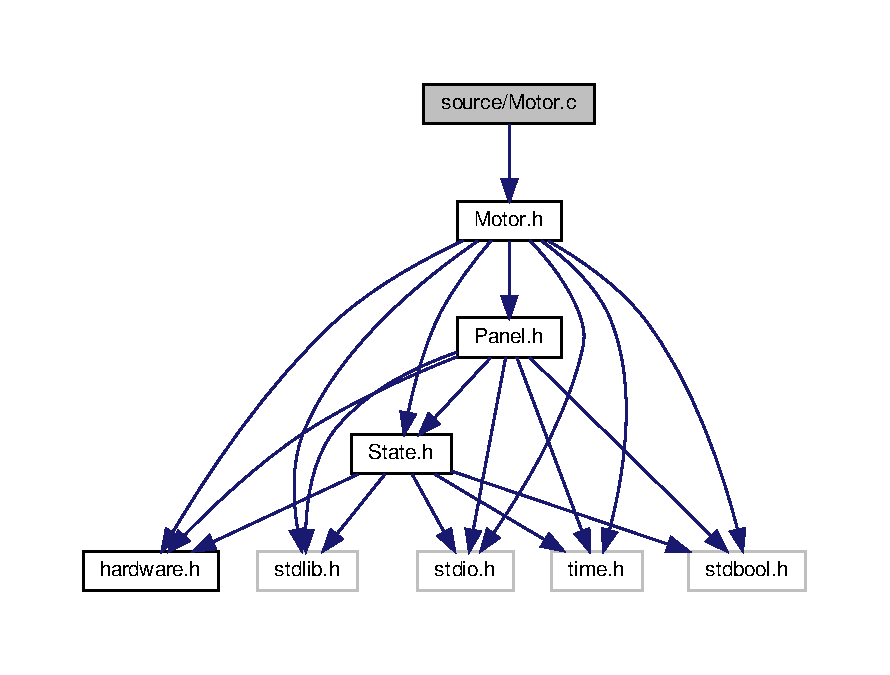
\includegraphics[width=350pt]{Motor_8c__incl}
\end{center}
\end{figure}
\subsection*{Functions}
\begin{DoxyCompactItemize}
\item 
\mbox{\Hypertarget{Motor_8c_ac0f5d349f7c8c7c1e994d04f4d9fd082}\label{Motor_8c_ac0f5d349f7c8c7c1e994d04f4d9fd082}} 
void \hyperlink{Motor_8c_ac0f5d349f7c8c7c1e994d04f4d9fd082}{elevator\+Drive} (\hyperlink{structPanel}{Panel} $\ast$p, \hyperlink{structState}{State} $\ast$s)
\begin{DoxyCompactList}\small\item\em elevator\+Drive main function for driving the elevator \end{DoxyCompactList}\end{DoxyCompactItemize}


\subsection{Detailed Description}
Struct and functionality to handle state of elevator. 


\hypertarget{Motor_8h}{}\section{source/\+Motor.h File Reference}
\label{Motor_8h}\index{source/\+Motor.\+h@{source/\+Motor.\+h}}


Functionality for driving the elevator.  


{\ttfamily \#include $<$stdio.\+h$>$}\newline
{\ttfamily \#include $<$stdlib.\+h$>$}\newline
{\ttfamily \#include $<$stdbool.\+h$>$}\newline
{\ttfamily \#include $<$time.\+h$>$}\newline
{\ttfamily \#include \char`\"{}hardware.\+h\char`\"{}}\newline
{\ttfamily \#include \char`\"{}State.\+h\char`\"{}}\newline
{\ttfamily \#include \char`\"{}Panel.\+h\char`\"{}}\newline
Include dependency graph for Motor.\+h\+:
\nopagebreak
\begin{figure}[H]
\begin{center}
\leavevmode
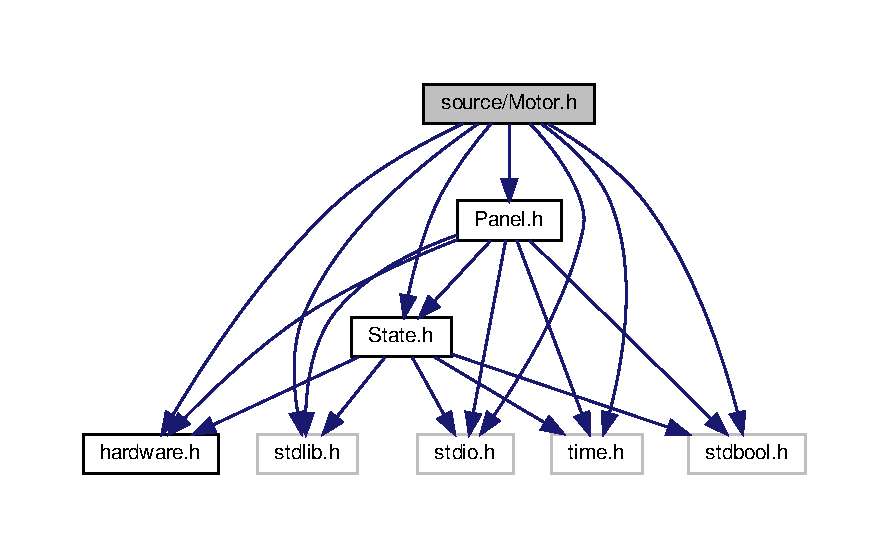
\includegraphics[width=350pt]{Motor_8h__incl}
\end{center}
\end{figure}
This graph shows which files directly or indirectly include this file\+:
\nopagebreak
\begin{figure}[H]
\begin{center}
\leavevmode
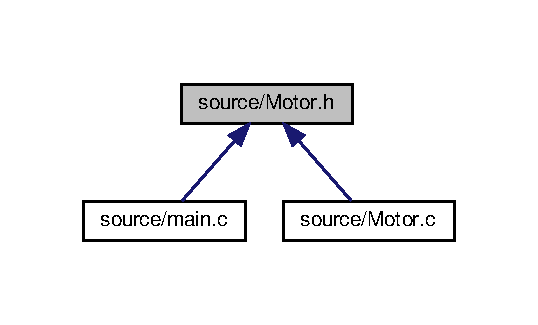
\includegraphics[width=258pt]{Motor_8h__dep__incl}
\end{center}
\end{figure}
\subsection*{Functions}
\begin{DoxyCompactItemize}
\item 
void \hyperlink{Motor_8h_ac0f5d349f7c8c7c1e994d04f4d9fd082}{elevator\+Drive} (\hyperlink{structPanel}{Panel} $\ast$p, \hyperlink{structState}{State} $\ast$s)
\begin{DoxyCompactList}\small\item\em Main function for driving the elevator. \end{DoxyCompactList}\end{DoxyCompactItemize}


\subsection{Detailed Description}
Functionality for driving the elevator. 



\subsection{Function Documentation}
\mbox{\Hypertarget{Motor_8h_ac0f5d349f7c8c7c1e994d04f4d9fd082}\label{Motor_8h_ac0f5d349f7c8c7c1e994d04f4d9fd082}} 
\index{Motor.\+h@{Motor.\+h}!elevator\+Drive@{elevator\+Drive}}
\index{elevator\+Drive@{elevator\+Drive}!Motor.\+h@{Motor.\+h}}
\subsubsection{\texorpdfstring{elevator\+Drive()}{elevatorDrive()}}
{\footnotesize\ttfamily void elevator\+Drive (\begin{DoxyParamCaption}\item[{\hyperlink{structPanel}{Panel} $\ast$}]{p,  }\item[{\hyperlink{structState}{State} $\ast$}]{s }\end{DoxyParamCaption})}



Main function for driving the elevator. 


\begin{DoxyParams}[1]{Parameters}
\mbox{\tt in}  & {\em p} & \hyperlink{structPanel}{Panel} for the elevator to drive \\
\hline
\mbox{\tt in}  & {\em s} & \hyperlink{structState}{State} of the elevator to drive \\
\hline
\end{DoxyParams}


Definition at line 8 of file Motor.\+c.


\hypertarget{Panel_8c}{}\section{source/\+Panel.c File Reference}
\label{Panel_8c}\index{source/\+Panel.\+c@{source/\+Panel.\+c}}


Implementation of \hyperlink{Panel_8h}{Panel.\+h}.  


{\ttfamily \#include \char`\"{}Panel.\+h\char`\"{}}\newline
Include dependency graph for Panel.\+c\+:
\nopagebreak
\begin{figure}[H]
\begin{center}
\leavevmode
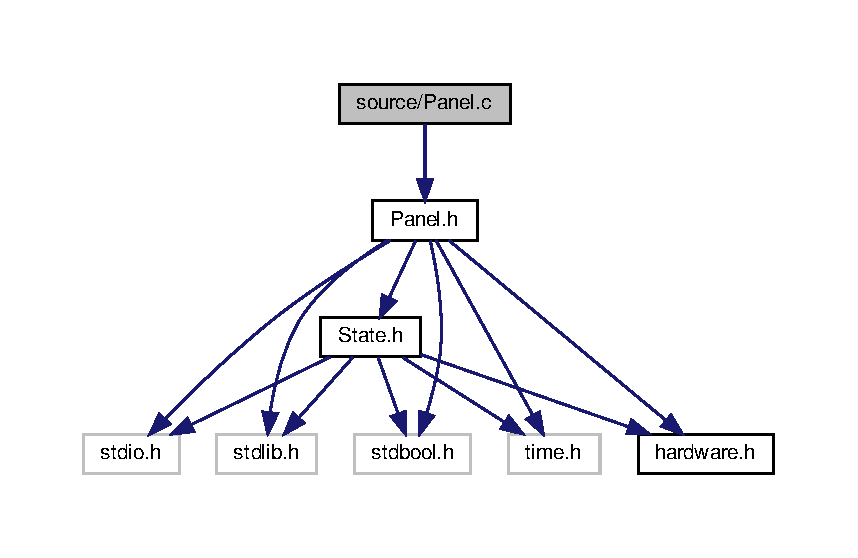
\includegraphics[width=350pt]{Panel_8c__incl}
\end{center}
\end{figure}
\subsection*{Functions}
\begin{DoxyCompactItemize}
\item 
\mbox{\Hypertarget{Panel_8c_acad85b10af5496b4552ead8241419793}\label{Panel_8c_acad85b10af5496b4552ead8241419793}} 
void \hyperlink{Panel_8c_acad85b10af5496b4552ead8241419793}{clean\+Orders} (int $\ast$orders)
\begin{DoxyCompactList}\small\item\em clean\+Orders function to clear all orders \end{DoxyCompactList}\item 
\mbox{\Hypertarget{Panel_8c_a03e8459eaa863a4c7e3a21985f407618}\label{Panel_8c_a03e8459eaa863a4c7e3a21985f407618}} 
void \hyperlink{Panel_8c_a03e8459eaa863a4c7e3a21985f407618}{panel\+Default} (\hyperlink{structPanel}{Panel} $\ast$p)
\begin{DoxyCompactList}\small\item\em panel\+Default function to initialize panel \end{DoxyCompactList}\item 
\mbox{\Hypertarget{Panel_8c_a5192947f9c6d4e31b11ae7afbc1800dc}\label{Panel_8c_a5192947f9c6d4e31b11ae7afbc1800dc}} 
int \hyperlink{Panel_8c_a5192947f9c6d4e31b11ae7afbc1800dc}{check\+Orders} (int $\ast$orders, int floor)
\begin{DoxyCompactList}\small\item\em check\+Orders function to check if order is already in array \end{DoxyCompactList}\item 
\mbox{\Hypertarget{Panel_8c_a0934eefc1f95dfa55dc0f800d5025d10}\label{Panel_8c_a0934eefc1f95dfa55dc0f800d5025d10}} 
void \hyperlink{Panel_8c_a0934eefc1f95dfa55dc0f800d5025d10}{left\+\_\+shift\+Orders} (int $\ast$orders)
\begin{DoxyCompactList}\small\item\em left\+\_\+shift\+Orders function to shift orders to the left side \end{DoxyCompactList}\item 
\mbox{\Hypertarget{Panel_8c_a1fd21468d55f6b120450c76aff0fa254}\label{Panel_8c_a1fd21468d55f6b120450c76aff0fa254}} 
void \hyperlink{Panel_8c_a1fd21468d55f6b120450c76aff0fa254}{push\+Orders} (\hyperlink{structPanel}{Panel} $\ast$p)
\begin{DoxyCompactList}\small\item\em push\+Orders function to push orders into orders array \end{DoxyCompactList}\item 
\mbox{\Hypertarget{Panel_8c_ab9707d9a622844ffc0b1ae1b77764aaa}\label{Panel_8c_ab9707d9a622844ffc0b1ae1b77764aaa}} 
void \hyperlink{Panel_8c_ab9707d9a622844ffc0b1ae1b77764aaa}{delay} (int number\+\_\+of\+\_\+seconds)
\begin{DoxyCompactList}\small\item\em delay function to add time-\/delay \end{DoxyCompactList}\item 
\mbox{\Hypertarget{Panel_8c_acd4f31281b2506ab5d009ffbf80f75da}\label{Panel_8c_acd4f31281b2506ab5d009ffbf80f75da}} 
bool \hyperlink{Panel_8c_acd4f31281b2506ab5d009ffbf80f75da}{check\+\_\+if\+\_\+orders} (\hyperlink{structPanel}{Panel} $\ast$p)
\begin{DoxyCompactList}\small\item\em check\+\_\+if\+\_\+orders function to check if there are orders in the orders array \end{DoxyCompactList}\item 
\mbox{\Hypertarget{Panel_8c_a14d66228d3632853c0dd0284abb93c32}\label{Panel_8c_a14d66228d3632853c0dd0284abb93c32}} 
int \hyperlink{Panel_8c_a14d66228d3632853c0dd0284abb93c32}{max\+Value} (\hyperlink{structPanel}{Panel} $\ast$p, \hyperlink{structState}{State} $\ast$s)
\begin{DoxyCompactList}\small\item\em max\+Value function to return highest value in orders array \end{DoxyCompactList}\item 
\mbox{\Hypertarget{Panel_8c_a058e0caf8945003a5acdef81b5f23f52}\label{Panel_8c_a058e0caf8945003a5acdef81b5f23f52}} 
int \hyperlink{Panel_8c_a058e0caf8945003a5acdef81b5f23f52}{min\+Value} (\hyperlink{structPanel}{Panel} $\ast$p, \hyperlink{structState}{State} $\ast$s)
\begin{DoxyCompactList}\small\item\em min\+Value function to return lowest value in orders array \end{DoxyCompactList}\item 
\mbox{\Hypertarget{Panel_8c_ada867e3dcf22c84eedf3b817670271dc}\label{Panel_8c_ada867e3dcf22c84eedf3b817670271dc}} 
bool \hyperlink{Panel_8c_ada867e3dcf22c84eedf3b817670271dc}{series\+\_\+of\+\_\+downs} (\hyperlink{structPanel}{Panel} $\ast$p)
\begin{DoxyCompactList}\small\item\em series\+\_\+of\+\_\+downs function to check if orders include a series of downward-\/orders \end{DoxyCompactList}\item 
\mbox{\Hypertarget{Panel_8c_a9360a1f76a37d2c36bf5b69248e7e822}\label{Panel_8c_a9360a1f76a37d2c36bf5b69248e7e822}} 
bool \hyperlink{Panel_8c_a9360a1f76a37d2c36bf5b69248e7e822}{series\+\_\+of\+\_\+ups} (\hyperlink{structPanel}{Panel} $\ast$p)
\begin{DoxyCompactList}\small\item\em series\+\_\+of\+\_\+ups function to check if orders include a series of upward-\/orders \end{DoxyCompactList}\item 
\mbox{\Hypertarget{Panel_8c_ac80a446f487d6ceb3b2ea4cddb2a7881}\label{Panel_8c_ac80a446f487d6ceb3b2ea4cddb2a7881}} 
int \hyperlink{Panel_8c_ac80a446f487d6ceb3b2ea4cddb2a7881}{closest\+Floor} (\hyperlink{structPanel}{Panel} $\ast$p, \hyperlink{structState}{State} $\ast$s)
\begin{DoxyCompactList}\small\item\em closest function to return next floor to go to \end{DoxyCompactList}\item 
\mbox{\Hypertarget{Panel_8c_a35a42e3c4897fed8fc3fe8993ccd8d4f}\label{Panel_8c_a35a42e3c4897fed8fc3fe8993ccd8d4f}} 
void \hyperlink{Panel_8c_a35a42e3c4897fed8fc3fe8993ccd8d4f}{clear\+Executed} (\hyperlink{structPanel}{Panel} $\ast$p, \hyperlink{structState}{State} $\ast$s)
\begin{DoxyCompactList}\small\item\em clear\+Executed function to clear executed orders \end{DoxyCompactList}\item 
\mbox{\Hypertarget{Panel_8c_ac551199759bbca39f38a41f0d80f9f07}\label{Panel_8c_ac551199759bbca39f38a41f0d80f9f07}} 
void \hyperlink{Panel_8c_ac551199759bbca39f38a41f0d80f9f07}{reached\+\_\+\+Floor} (\hyperlink{structPanel}{Panel} $\ast$p, \hyperlink{structState}{State} $\ast$s)
\begin{DoxyCompactList}\small\item\em reached\+\_\+\+Floor function to check if elevator has reached the correct floor \end{DoxyCompactList}\end{DoxyCompactItemize}


\subsection{Detailed Description}
Implementation of \hyperlink{Panel_8h}{Panel.\+h}. 


\hypertarget{Panel_8h}{}\section{source/\+Panel.h File Reference}
\label{Panel_8h}\index{source/\+Panel.\+h@{source/\+Panel.\+h}}


Functionality in conjunction with elevator panel.  


{\ttfamily \#include $<$stdio.\+h$>$}\newline
{\ttfamily \#include $<$stdlib.\+h$>$}\newline
{\ttfamily \#include $<$stdbool.\+h$>$}\newline
{\ttfamily \#include $<$time.\+h$>$}\newline
{\ttfamily \#include \char`\"{}hardware.\+h\char`\"{}}\newline
{\ttfamily \#include \char`\"{}State.\+h\char`\"{}}\newline
Include dependency graph for Panel.\+h\+:\nopagebreak
\begin{figure}[H]
\begin{center}
\leavevmode
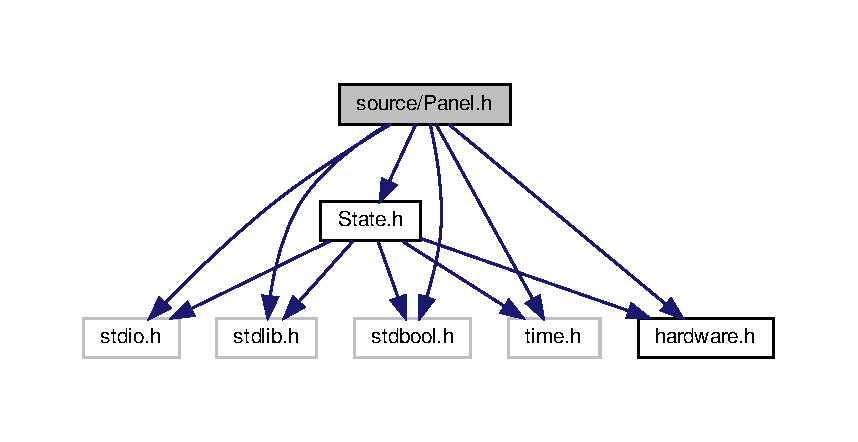
\includegraphics[width=350pt]{Panel_8h__incl}
\end{center}
\end{figure}
This graph shows which files directly or indirectly include this file\+:
\nopagebreak
\begin{figure}[H]
\begin{center}
\leavevmode
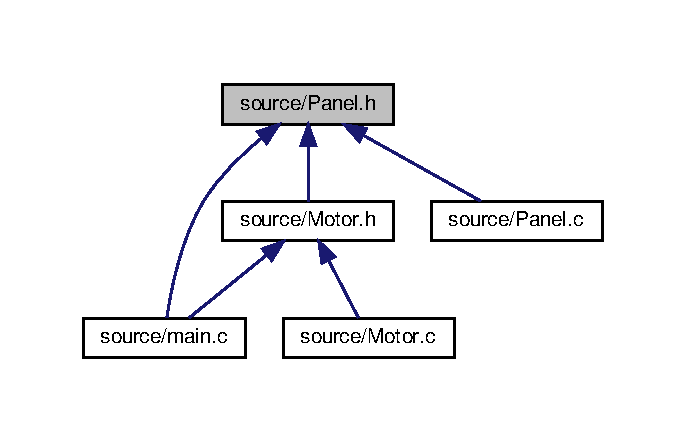
\includegraphics[width=329pt]{Panel_8h__dep__incl}
\end{center}
\end{figure}
\subsection*{Data Structures}
\begin{DoxyCompactItemize}
\item 
struct \hyperlink{structPanel}{Panel}
\begin{DoxyCompactList}\small\item\em Struct to contain information about buttons pushed on elevator panels. \end{DoxyCompactList}\end{DoxyCompactItemize}
\subsection*{Enumerations}
\begin{DoxyCompactItemize}
\item 
\mbox{\Hypertarget{Panel_8h_ab89626a4ae8bd4e703ae46ce88cfb490}\label{Panel_8h_ab89626a4ae8bd4e703ae46ce88cfb490}} 
enum \hyperlink{Panel_8h_ab89626a4ae8bd4e703ae46ce88cfb490}{O\+R\+D\+E\+R\+T\+Y\+PE} \{ {\bfseries O\+R\+D\+E\+R\+\_\+\+UP} = 1, 
{\bfseries O\+R\+D\+E\+R\+\_\+\+I\+N\+S\+I\+DE} = 0, 
{\bfseries O\+R\+D\+E\+R\+\_\+\+D\+O\+WN} = -\/1
 \}\begin{DoxyCompactList}\small\item\em Enum containing numbers according to type of order. \end{DoxyCompactList}
\end{DoxyCompactItemize}
\subsection*{Functions}
\begin{DoxyCompactItemize}
\item 
void \hyperlink{Panel_8h_acad85b10af5496b4552ead8241419793}{clean\+Orders} (int $\ast$orders)
\begin{DoxyCompactList}\small\item\em Function to clear all orders. \end{DoxyCompactList}\item 
int \hyperlink{Panel_8h_a5192947f9c6d4e31b11ae7afbc1800dc}{check\+Orders} (int $\ast$orders, int floor)
\begin{DoxyCompactList}\small\item\em Function to check if order is already in array, return -\/1 if not. \end{DoxyCompactList}\item 
void \hyperlink{Panel_8h_a03e8459eaa863a4c7e3a21985f407618}{panel\+Default} (\hyperlink{structPanel}{Panel} $\ast$p)
\begin{DoxyCompactList}\small\item\em Function to initialize panel. \end{DoxyCompactList}\item 
void \hyperlink{Panel_8h_a6e33d972d9ef96e4ea43c0a1e8445b3d}{ls\+Orders} (int $\ast$orders)
\begin{DoxyCompactList}\small\item\em Function to shift orders to the left side. \end{DoxyCompactList}\item 
void \hyperlink{Panel_8h_a1fd21468d55f6b120450c76aff0fa254}{push\+Orders} (\hyperlink{structPanel}{Panel} $\ast$p)
\begin{DoxyCompactList}\small\item\em Function to push orders into orders array. \end{DoxyCompactList}\item 
void \hyperlink{Panel_8h_a6b9f3a7f61812553cbb6fb9df5e21620}{delay} (\hyperlink{structPanel}{Panel} $\ast$p, int number\+\_\+of\+\_\+seconds)
\begin{DoxyCompactList}\small\item\em Function to add time-\/delay and be able to push orders while in delay. \end{DoxyCompactList}\item 
int \hyperlink{Panel_8h_a14d66228d3632853c0dd0284abb93c32}{max\+Value} (\hyperlink{structPanel}{Panel} $\ast$p, \hyperlink{structState}{State} $\ast$s)
\begin{DoxyCompactList}\small\item\em Function to return highest value in orders array. \end{DoxyCompactList}\item 
int \hyperlink{Panel_8h_a058e0caf8945003a5acdef81b5f23f52}{min\+Value} (\hyperlink{structPanel}{Panel} $\ast$p, \hyperlink{structState}{State} $\ast$s)
\begin{DoxyCompactList}\small\item\em Function to return lowest value in orders array. \end{DoxyCompactList}\item 
bool \hyperlink{Panel_8h_a827423f0036ddebf7fb5bb1f3b64d6ed}{series\+Of\+Downs} (\hyperlink{structPanel}{Panel} $\ast$p)
\begin{DoxyCompactList}\small\item\em series\+Of\+Downs function to check if orders include a series of downward-\/orders (return true if there is) \end{DoxyCompactList}\item 
bool \hyperlink{Panel_8h_aa2b311278cea18199e1a55db260ba7aa}{series\+Of\+Ups} (\hyperlink{structPanel}{Panel} $\ast$p)
\begin{DoxyCompactList}\small\item\em series\+Of\+Ups function to check if orders include a series of upward-\/orders (return true if there is) \end{DoxyCompactList}\item 
int \hyperlink{Panel_8h_ac80a446f487d6ceb3b2ea4cddb2a7881}{closest\+Floor} (\hyperlink{structPanel}{Panel} $\ast$p, \hyperlink{structState}{State} $\ast$s)
\begin{DoxyCompactList}\small\item\em Function to return next floor to go to. \end{DoxyCompactList}\item 
void \hyperlink{Panel_8h_a35a42e3c4897fed8fc3fe8993ccd8d4f}{clear\+Executed} (\hyperlink{structPanel}{Panel} $\ast$p, \hyperlink{structState}{State} $\ast$s)
\begin{DoxyCompactList}\small\item\em Function to clear executed orders. \end{DoxyCompactList}\item 
void \hyperlink{Panel_8h_a4dbf04c3a78cd52c02b19fc71715dcf3}{floor\+Reached} (\hyperlink{structPanel}{Panel} $\ast$p, \hyperlink{structState}{State} $\ast$s)
\begin{DoxyCompactList}\small\item\em Function to check if elevator has reached the correct floor. \end{DoxyCompactList}\item 
bool \hyperlink{Panel_8h_acac36c822c1bf712637a7e349ec0ef65}{check\+If\+Orders} (\hyperlink{structPanel}{Panel} $\ast$p)
\begin{DoxyCompactList}\small\item\em Function to check if there are orders in the orders array. \end{DoxyCompactList}\item 
void \hyperlink{Panel_8h_a2ae86946a1d05353e57e5b3fb7785989}{set\+Order\+Lights} (\hyperlink{structPanel}{Panel} $\ast$p)
\begin{DoxyCompactList}\small\item\em Function to set order lights. \end{DoxyCompactList}\end{DoxyCompactItemize}


\subsection{Detailed Description}
Functionality in conjunction with elevator panel. 



\subsection{Function Documentation}
\mbox{\Hypertarget{Panel_8h_acac36c822c1bf712637a7e349ec0ef65}\label{Panel_8h_acac36c822c1bf712637a7e349ec0ef65}} 
\index{Panel.\+h@{Panel.\+h}!check\+If\+Orders@{check\+If\+Orders}}
\index{check\+If\+Orders@{check\+If\+Orders}!Panel.\+h@{Panel.\+h}}
\subsubsection{\texorpdfstring{check\+If\+Orders()}{checkIfOrders()}}
{\footnotesize\ttfamily bool check\+If\+Orders (\begin{DoxyParamCaption}\item[{\hyperlink{structPanel}{Panel} $\ast$}]{p }\end{DoxyParamCaption})}



Function to check if there are orders in the orders array. 


\begin{DoxyParams}[1]{Parameters}
\mbox{\tt in}  & {\em p} & \hyperlink{structPanel}{Panel} containing orders to check out \\
\hline
\end{DoxyParams}


Definition at line 113 of file Panel.\+c.

\mbox{\Hypertarget{Panel_8h_a5192947f9c6d4e31b11ae7afbc1800dc}\label{Panel_8h_a5192947f9c6d4e31b11ae7afbc1800dc}} 
\index{Panel.\+h@{Panel.\+h}!check\+Orders@{check\+Orders}}
\index{check\+Orders@{check\+Orders}!Panel.\+h@{Panel.\+h}}
\subsubsection{\texorpdfstring{check\+Orders()}{checkOrders()}}
{\footnotesize\ttfamily int check\+Orders (\begin{DoxyParamCaption}\item[{int $\ast$}]{orders,  }\item[{int}]{floor }\end{DoxyParamCaption})}



Function to check if order is already in array, return -\/1 if not. 


\begin{DoxyParams}[1]{Parameters}
\mbox{\tt in}  & {\em orders} & Array of orders \\
\hline
\mbox{\tt in}  & {\em floor} & Floor to check \\
\hline
\end{DoxyParams}


Definition at line 28 of file Panel.\+c.

\mbox{\Hypertarget{Panel_8h_acad85b10af5496b4552ead8241419793}\label{Panel_8h_acad85b10af5496b4552ead8241419793}} 
\index{Panel.\+h@{Panel.\+h}!clean\+Orders@{clean\+Orders}}
\index{clean\+Orders@{clean\+Orders}!Panel.\+h@{Panel.\+h}}
\subsubsection{\texorpdfstring{clean\+Orders()}{cleanOrders()}}
{\footnotesize\ttfamily void clean\+Orders (\begin{DoxyParamCaption}\item[{int $\ast$}]{orders }\end{DoxyParamCaption})}



Function to clear all orders. 


\begin{DoxyParams}[1]{Parameters}
\mbox{\tt in}  & {\em orders} & Array of orders \\
\hline
\end{DoxyParams}


Definition at line 8 of file Panel.\+c.

\mbox{\Hypertarget{Panel_8h_a35a42e3c4897fed8fc3fe8993ccd8d4f}\label{Panel_8h_a35a42e3c4897fed8fc3fe8993ccd8d4f}} 
\index{Panel.\+h@{Panel.\+h}!clear\+Executed@{clear\+Executed}}
\index{clear\+Executed@{clear\+Executed}!Panel.\+h@{Panel.\+h}}
\subsubsection{\texorpdfstring{clear\+Executed()}{clearExecuted()}}
{\footnotesize\ttfamily void clear\+Executed (\begin{DoxyParamCaption}\item[{\hyperlink{structPanel}{Panel} $\ast$}]{p,  }\item[{\hyperlink{structState}{State} $\ast$}]{s }\end{DoxyParamCaption})}



Function to clear executed orders. 


\begin{DoxyParams}[1]{Parameters}
\mbox{\tt in}  & {\em p} & \hyperlink{structPanel}{Panel} containing executed orders to clear \\
\hline
\mbox{\tt in}  & {\em s} & \hyperlink{structState}{State} of elevator \\
\hline
\end{DoxyParams}


Definition at line 214 of file Panel.\+c.

\mbox{\Hypertarget{Panel_8h_ac80a446f487d6ceb3b2ea4cddb2a7881}\label{Panel_8h_ac80a446f487d6ceb3b2ea4cddb2a7881}} 
\index{Panel.\+h@{Panel.\+h}!closest\+Floor@{closest\+Floor}}
\index{closest\+Floor@{closest\+Floor}!Panel.\+h@{Panel.\+h}}
\subsubsection{\texorpdfstring{closest\+Floor()}{closestFloor()}}
{\footnotesize\ttfamily int closest\+Floor (\begin{DoxyParamCaption}\item[{\hyperlink{structPanel}{Panel} $\ast$}]{p,  }\item[{\hyperlink{structState}{State} $\ast$}]{s }\end{DoxyParamCaption})}



Function to return next floor to go to. 


\begin{DoxyParams}[1]{Parameters}
\mbox{\tt in}  & {\em p} & \hyperlink{structPanel}{Panel} containing orders to check out \\
\hline
\mbox{\tt in}  & {\em s} & \hyperlink{structState}{State} of elevator \\
\hline
\end{DoxyParams}


Definition at line 173 of file Panel.\+c.

\mbox{\Hypertarget{Panel_8h_a6b9f3a7f61812553cbb6fb9df5e21620}\label{Panel_8h_a6b9f3a7f61812553cbb6fb9df5e21620}} 
\index{Panel.\+h@{Panel.\+h}!delay@{delay}}
\index{delay@{delay}!Panel.\+h@{Panel.\+h}}
\subsubsection{\texorpdfstring{delay()}{delay()}}
{\footnotesize\ttfamily void delay (\begin{DoxyParamCaption}\item[{\hyperlink{structPanel}{Panel} $\ast$}]{p,  }\item[{int}]{number\+\_\+of\+\_\+seconds }\end{DoxyParamCaption})}



Function to add time-\/delay and be able to push orders while in delay. 


\begin{DoxyParams}[1]{Parameters}
\mbox{\tt in}  & {\em p} & \hyperlink{structPanel}{Panel} to push orders into while in delay \\
\hline
\mbox{\tt in}  & {\em number\+\_\+of\+\_\+seconds} & Number of seconds to delay \\
\hline
\end{DoxyParams}


Definition at line 96 of file Panel.\+c.

\mbox{\Hypertarget{Panel_8h_a4dbf04c3a78cd52c02b19fc71715dcf3}\label{Panel_8h_a4dbf04c3a78cd52c02b19fc71715dcf3}} 
\index{Panel.\+h@{Panel.\+h}!floor\+Reached@{floor\+Reached}}
\index{floor\+Reached@{floor\+Reached}!Panel.\+h@{Panel.\+h}}
\subsubsection{\texorpdfstring{floor\+Reached()}{floorReached()}}
{\footnotesize\ttfamily void floor\+Reached (\begin{DoxyParamCaption}\item[{\hyperlink{structPanel}{Panel} $\ast$}]{p,  }\item[{\hyperlink{structState}{State} $\ast$}]{s }\end{DoxyParamCaption})}



Function to check if elevator has reached the correct floor. 


\begin{DoxyParams}[1]{Parameters}
\mbox{\tt in}  & {\em p} & \hyperlink{structPanel}{Panel} containing orders to check out \\
\hline
\mbox{\tt in}  & {\em s} & \hyperlink{structState}{State} of elevator \\
\hline
\end{DoxyParams}


Definition at line 231 of file Panel.\+c.

\mbox{\Hypertarget{Panel_8h_a6e33d972d9ef96e4ea43c0a1e8445b3d}\label{Panel_8h_a6e33d972d9ef96e4ea43c0a1e8445b3d}} 
\index{Panel.\+h@{Panel.\+h}!ls\+Orders@{ls\+Orders}}
\index{ls\+Orders@{ls\+Orders}!Panel.\+h@{Panel.\+h}}
\subsubsection{\texorpdfstring{ls\+Orders()}{lsOrders()}}
{\footnotesize\ttfamily void ls\+Orders (\begin{DoxyParamCaption}\item[{int $\ast$}]{orders }\end{DoxyParamCaption})}



Function to shift orders to the left side. 


\begin{DoxyParams}[1]{Parameters}
\mbox{\tt in}  & {\em orders} & Array to leftshift \\
\hline
\end{DoxyParams}


Definition at line 38 of file Panel.\+c.

\mbox{\Hypertarget{Panel_8h_a14d66228d3632853c0dd0284abb93c32}\label{Panel_8h_a14d66228d3632853c0dd0284abb93c32}} 
\index{Panel.\+h@{Panel.\+h}!max\+Value@{max\+Value}}
\index{max\+Value@{max\+Value}!Panel.\+h@{Panel.\+h}}
\subsubsection{\texorpdfstring{max\+Value()}{maxValue()}}
{\footnotesize\ttfamily int max\+Value (\begin{DoxyParamCaption}\item[{\hyperlink{structPanel}{Panel} $\ast$}]{p,  }\item[{\hyperlink{structState}{State} $\ast$}]{s }\end{DoxyParamCaption})}



Function to return highest value in orders array. 


\begin{DoxyParams}[1]{Parameters}
\mbox{\tt in}  & {\em p} & \hyperlink{structPanel}{Panel} containing orders to check out \\
\hline
\mbox{\tt in}  & {\em s} & \hyperlink{structState}{State} of elevator \\
\hline
\end{DoxyParams}


Definition at line 122 of file Panel.\+c.

\mbox{\Hypertarget{Panel_8h_a058e0caf8945003a5acdef81b5f23f52}\label{Panel_8h_a058e0caf8945003a5acdef81b5f23f52}} 
\index{Panel.\+h@{Panel.\+h}!min\+Value@{min\+Value}}
\index{min\+Value@{min\+Value}!Panel.\+h@{Panel.\+h}}
\subsubsection{\texorpdfstring{min\+Value()}{minValue()}}
{\footnotesize\ttfamily int min\+Value (\begin{DoxyParamCaption}\item[{\hyperlink{structPanel}{Panel} $\ast$}]{p,  }\item[{\hyperlink{structState}{State} $\ast$}]{s }\end{DoxyParamCaption})}



Function to return lowest value in orders array. 


\begin{DoxyParams}[1]{Parameters}
\mbox{\tt in}  & {\em p} & \hyperlink{structPanel}{Panel} containing orders to check out \\
\hline
\mbox{\tt in}  & {\em s} & \hyperlink{structState}{State} of elevator \\
\hline
\end{DoxyParams}


Definition at line 137 of file Panel.\+c.

\mbox{\Hypertarget{Panel_8h_a03e8459eaa863a4c7e3a21985f407618}\label{Panel_8h_a03e8459eaa863a4c7e3a21985f407618}} 
\index{Panel.\+h@{Panel.\+h}!panel\+Default@{panel\+Default}}
\index{panel\+Default@{panel\+Default}!Panel.\+h@{Panel.\+h}}
\subsubsection{\texorpdfstring{panel\+Default()}{panelDefault()}}
{\footnotesize\ttfamily void panel\+Default (\begin{DoxyParamCaption}\item[{\hyperlink{structPanel}{Panel} $\ast$}]{p }\end{DoxyParamCaption})}



Function to initialize panel. 


\begin{DoxyParams}[1]{Parameters}
\mbox{\tt in}  & {\em p} & \hyperlink{structPanel}{Panel} to initialize \\
\hline
\end{DoxyParams}


Definition at line 21 of file Panel.\+c.

\mbox{\Hypertarget{Panel_8h_a1fd21468d55f6b120450c76aff0fa254}\label{Panel_8h_a1fd21468d55f6b120450c76aff0fa254}} 
\index{Panel.\+h@{Panel.\+h}!push\+Orders@{push\+Orders}}
\index{push\+Orders@{push\+Orders}!Panel.\+h@{Panel.\+h}}
\subsubsection{\texorpdfstring{push\+Orders()}{pushOrders()}}
{\footnotesize\ttfamily void push\+Orders (\begin{DoxyParamCaption}\item[{\hyperlink{structPanel}{Panel} $\ast$}]{p }\end{DoxyParamCaption})}



Function to push orders into orders array. 


\begin{DoxyParams}[1]{Parameters}
\mbox{\tt in}  & {\em p} & \hyperlink{structPanel}{Panel} to push orders into \\
\hline
\end{DoxyParams}


Definition at line 52 of file Panel.\+c.

\mbox{\Hypertarget{Panel_8h_a827423f0036ddebf7fb5bb1f3b64d6ed}\label{Panel_8h_a827423f0036ddebf7fb5bb1f3b64d6ed}} 
\index{Panel.\+h@{Panel.\+h}!series\+Of\+Downs@{series\+Of\+Downs}}
\index{series\+Of\+Downs@{series\+Of\+Downs}!Panel.\+h@{Panel.\+h}}
\subsubsection{\texorpdfstring{series\+Of\+Downs()}{seriesOfDowns()}}
{\footnotesize\ttfamily bool series\+Of\+Downs (\begin{DoxyParamCaption}\item[{\hyperlink{structPanel}{Panel} $\ast$}]{p }\end{DoxyParamCaption})}



series\+Of\+Downs function to check if orders include a series of downward-\/orders (return true if there is) 


\begin{DoxyParams}[1]{Parameters}
\mbox{\tt in}  & {\em p} & \hyperlink{structPanel}{Panel} containing orders to check out \\
\hline
\end{DoxyParams}


Definition at line 151 of file Panel.\+c.

\mbox{\Hypertarget{Panel_8h_aa2b311278cea18199e1a55db260ba7aa}\label{Panel_8h_aa2b311278cea18199e1a55db260ba7aa}} 
\index{Panel.\+h@{Panel.\+h}!series\+Of\+Ups@{series\+Of\+Ups}}
\index{series\+Of\+Ups@{series\+Of\+Ups}!Panel.\+h@{Panel.\+h}}
\subsubsection{\texorpdfstring{series\+Of\+Ups()}{seriesOfUps()}}
{\footnotesize\ttfamily bool series\+Of\+Ups (\begin{DoxyParamCaption}\item[{\hyperlink{structPanel}{Panel} $\ast$}]{p }\end{DoxyParamCaption})}



series\+Of\+Ups function to check if orders include a series of upward-\/orders (return true if there is) 


\begin{DoxyParams}[1]{Parameters}
\mbox{\tt in}  & {\em p} & \hyperlink{structPanel}{Panel} containing orders to check out \\
\hline
\end{DoxyParams}


Definition at line 162 of file Panel.\+c.

\mbox{\Hypertarget{Panel_8h_a2ae86946a1d05353e57e5b3fb7785989}\label{Panel_8h_a2ae86946a1d05353e57e5b3fb7785989}} 
\index{Panel.\+h@{Panel.\+h}!set\+Order\+Lights@{set\+Order\+Lights}}
\index{set\+Order\+Lights@{set\+Order\+Lights}!Panel.\+h@{Panel.\+h}}
\subsubsection{\texorpdfstring{set\+Order\+Lights()}{setOrderLights()}}
{\footnotesize\ttfamily void set\+Order\+Lights (\begin{DoxyParamCaption}\item[{\hyperlink{structPanel}{Panel} $\ast$}]{p }\end{DoxyParamCaption})}



Function to set order lights. 


\begin{DoxyParams}[1]{Parameters}
\mbox{\tt in}  & {\em p} & \hyperlink{structPanel}{Panel} containing orders we want to turn on lights for \\
\hline
\end{DoxyParams}


Definition at line 245 of file Panel.\+c.


\hypertarget{State_8c}{}\section{source/\+State.c File Reference}
\label{State_8c}\index{source/\+State.\+c@{source/\+State.\+c}}


Implementation of \hyperlink{State_8h}{State.\+h}.  


{\ttfamily \#include \char`\"{}State.\+h\char`\"{}}\newline
Include dependency graph for State.\+c\+:\nopagebreak
\begin{figure}[H]
\begin{center}
\leavevmode
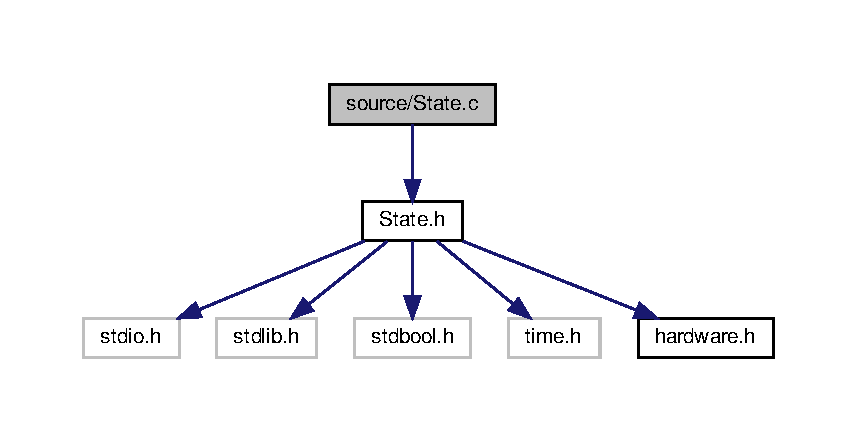
\includegraphics[width=350pt]{State_8c__incl}
\end{center}
\end{figure}
\subsection*{Functions}
\begin{DoxyCompactItemize}
\item 
void \hyperlink{State_8c_aeeb7819b7b73579cb65b2258d43004b3}{state\+Default} (\hyperlink{structState}{State} $\ast$Elevator)
\begin{DoxyCompactList}\small\item\em Function to initialize state of elevator (use only outside of while-\/loop) \end{DoxyCompactList}\item 
\mbox{\Hypertarget{State_8c_a90f96e4c6bcd783cbd2dc2addf39b803}\label{State_8c_a90f96e4c6bcd783cbd2dc2addf39b803}} 
int \hyperlink{State_8c_a90f96e4c6bcd783cbd2dc2addf39b803}{check\+State} ()
\begin{DoxyCompactList}\small\item\em Function to check if elevator is in a defined state (returns 1 if it is, 0 if not) \end{DoxyCompactList}\item 
int \hyperlink{State_8c_ad3aa6fc318fede39e5889b004ec47be0}{get\+Floor} (int check)
\begin{DoxyCompactList}\small\item\em Function to return the floor elevator is in (needs to be in a defined state to return anything) \end{DoxyCompactList}\item 
void \hyperlink{State_8c_a62c85e3e21ac96c3aaadc46219e17dca}{state\+Control} (\hyperlink{structState}{State} $\ast$Elevator)
\begin{DoxyCompactList}\small\item\em Function to update the state of elevator throughout the loop. \end{DoxyCompactList}\end{DoxyCompactItemize}


\subsection{Detailed Description}
Implementation of \hyperlink{State_8h}{State.\+h}. 



\subsection{Function Documentation}
\mbox{\Hypertarget{State_8c_ad3aa6fc318fede39e5889b004ec47be0}\label{State_8c_ad3aa6fc318fede39e5889b004ec47be0}} 
\index{State.\+c@{State.\+c}!get\+Floor@{get\+Floor}}
\index{get\+Floor@{get\+Floor}!State.\+c@{State.\+c}}
\subsubsection{\texorpdfstring{get\+Floor()}{getFloor()}}
{\footnotesize\ttfamily int get\+Floor (\begin{DoxyParamCaption}\item[{int}]{check }\end{DoxyParamCaption})}



Function to return the floor elevator is in (needs to be in a defined state to return anything) 


\begin{DoxyParams}[1]{Parameters}
\mbox{\tt in}  & {\em check} & Parameter to tell function if elevator is in a defined state \\
\hline
\end{DoxyParams}


Definition at line 40 of file State.\+c.

\mbox{\Hypertarget{State_8c_a62c85e3e21ac96c3aaadc46219e17dca}\label{State_8c_a62c85e3e21ac96c3aaadc46219e17dca}} 
\index{State.\+c@{State.\+c}!state\+Control@{state\+Control}}
\index{state\+Control@{state\+Control}!State.\+c@{State.\+c}}
\subsubsection{\texorpdfstring{state\+Control()}{stateControl()}}
{\footnotesize\ttfamily void state\+Control (\begin{DoxyParamCaption}\item[{\hyperlink{structState}{State} $\ast$}]{Elevator }\end{DoxyParamCaption})}



Function to update the state of elevator throughout the loop. 


\begin{DoxyParams}[1]{Parameters}
\mbox{\tt in}  & {\em Elevator} & Elevator to follow state of \\
\hline
\end{DoxyParams}


Definition at line 52 of file State.\+c.

\mbox{\Hypertarget{State_8c_aeeb7819b7b73579cb65b2258d43004b3}\label{State_8c_aeeb7819b7b73579cb65b2258d43004b3}} 
\index{State.\+c@{State.\+c}!state\+Default@{state\+Default}}
\index{state\+Default@{state\+Default}!State.\+c@{State.\+c}}
\subsubsection{\texorpdfstring{state\+Default()}{stateDefault()}}
{\footnotesize\ttfamily void state\+Default (\begin{DoxyParamCaption}\item[{\hyperlink{structState}{State} $\ast$}]{Elevator }\end{DoxyParamCaption})}



Function to initialize state of elevator (use only outside of while-\/loop) 


\begin{DoxyParams}[1]{Parameters}
\mbox{\tt in}  & {\em Elevator} & Elevator to initialize \\
\hline
\end{DoxyParams}


Definition at line 8 of file State.\+c.


\hypertarget{State_8h}{}\section{source/\+State.h File Reference}
\label{State_8h}\index{source/\+State.\+h@{source/\+State.\+h}}


Struct and functionality to handle state of elevator.  


{\ttfamily \#include $<$stdio.\+h$>$}\newline
{\ttfamily \#include $<$stdlib.\+h$>$}\newline
{\ttfamily \#include $<$stdbool.\+h$>$}\newline
{\ttfamily \#include $<$time.\+h$>$}\newline
{\ttfamily \#include \char`\"{}hardware.\+h\char`\"{}}\newline
Include dependency graph for State.\+h\+:\nopagebreak
\begin{figure}[H]
\begin{center}
\leavevmode
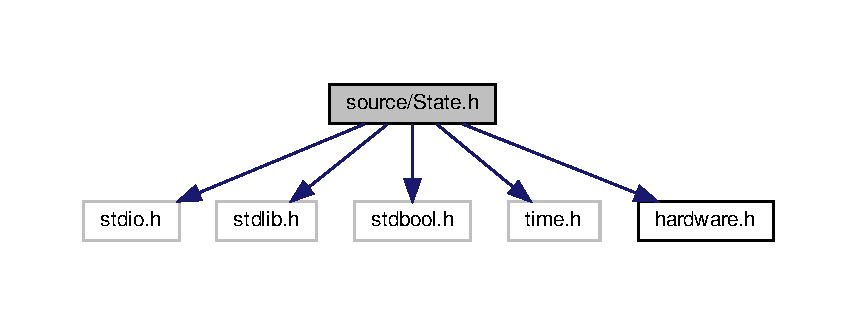
\includegraphics[width=350pt]{State_8h__incl}
\end{center}
\end{figure}
This graph shows which files directly or indirectly include this file\+:
\nopagebreak
\begin{figure}[H]
\begin{center}
\leavevmode
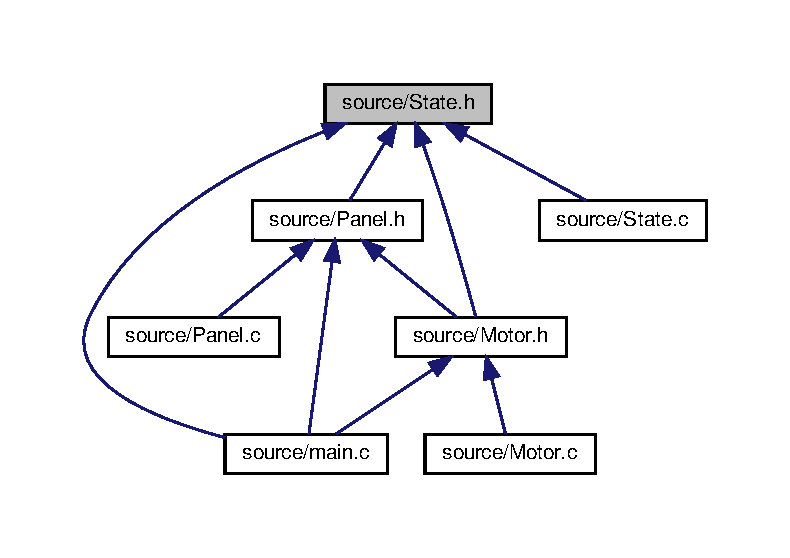
\includegraphics[width=350pt]{State_8h__dep__incl}
\end{center}
\end{figure}
\subsection*{Data Structures}
\begin{DoxyCompactItemize}
\item 
struct \hyperlink{structState}{State}
\begin{DoxyCompactList}\small\item\em clean\+Orders function to clear all orders \end{DoxyCompactList}\end{DoxyCompactItemize}
\subsection*{Enumerations}
\begin{DoxyCompactItemize}
\item 
\mbox{\Hypertarget{State_8h_aa268a41a13430b18e933ed40207178d0}\label{State_8h_aa268a41a13430b18e933ed40207178d0}} 
enum \hyperlink{State_8h_aa268a41a13430b18e933ed40207178d0}{D\+I\+R\+E\+C\+T\+I\+ON} \{ {\bfseries UP} = 1, 
{\bfseries S\+T\+OP} = 0, 
{\bfseries D\+O\+WN} = -\/1
 \}\begin{DoxyCompactList}\small\item\em Enum containg values for elevator direction. \end{DoxyCompactList}
\end{DoxyCompactItemize}
\subsection*{Functions}
\begin{DoxyCompactItemize}
\item 
void \hyperlink{State_8h_aeeb7819b7b73579cb65b2258d43004b3}{state\+Default} (\hyperlink{structState}{State} $\ast$Elevator)
\begin{DoxyCompactList}\small\item\em Function to initialize state of elevator (use only outside of while-\/loop) \end{DoxyCompactList}\item 
\mbox{\Hypertarget{State_8h_a90f96e4c6bcd783cbd2dc2addf39b803}\label{State_8h_a90f96e4c6bcd783cbd2dc2addf39b803}} 
int \hyperlink{State_8h_a90f96e4c6bcd783cbd2dc2addf39b803}{check\+State} ()
\begin{DoxyCompactList}\small\item\em Function to check if elevator is in a defined state (returns 1 if it is, 0 if not) \end{DoxyCompactList}\item 
int \hyperlink{State_8h_ad3aa6fc318fede39e5889b004ec47be0}{get\+Floor} (int check)
\begin{DoxyCompactList}\small\item\em Function to return the floor elevator is in (needs to be in a defined state to return anything) \end{DoxyCompactList}\item 
void \hyperlink{State_8h_a62c85e3e21ac96c3aaadc46219e17dca}{state\+Control} (\hyperlink{structState}{State} $\ast$Elevator)
\begin{DoxyCompactList}\small\item\em Function to update the state of elevator throughout the loop. \end{DoxyCompactList}\end{DoxyCompactItemize}


\subsection{Detailed Description}
Struct and functionality to handle state of elevator. 



\subsection{Function Documentation}
\mbox{\Hypertarget{State_8h_ad3aa6fc318fede39e5889b004ec47be0}\label{State_8h_ad3aa6fc318fede39e5889b004ec47be0}} 
\index{State.\+h@{State.\+h}!get\+Floor@{get\+Floor}}
\index{get\+Floor@{get\+Floor}!State.\+h@{State.\+h}}
\subsubsection{\texorpdfstring{get\+Floor()}{getFloor()}}
{\footnotesize\ttfamily int get\+Floor (\begin{DoxyParamCaption}\item[{int}]{check }\end{DoxyParamCaption})}



Function to return the floor elevator is in (needs to be in a defined state to return anything) 


\begin{DoxyParams}[1]{Parameters}
\mbox{\tt in}  & {\em check} & Parameter to tell function if elevator is in a defined state \\
\hline
\end{DoxyParams}


Definition at line 40 of file State.\+c.

\mbox{\Hypertarget{State_8h_a62c85e3e21ac96c3aaadc46219e17dca}\label{State_8h_a62c85e3e21ac96c3aaadc46219e17dca}} 
\index{State.\+h@{State.\+h}!state\+Control@{state\+Control}}
\index{state\+Control@{state\+Control}!State.\+h@{State.\+h}}
\subsubsection{\texorpdfstring{state\+Control()}{stateControl()}}
{\footnotesize\ttfamily void state\+Control (\begin{DoxyParamCaption}\item[{\hyperlink{structState}{State} $\ast$}]{Elevator }\end{DoxyParamCaption})}



Function to update the state of elevator throughout the loop. 


\begin{DoxyParams}[1]{Parameters}
\mbox{\tt in}  & {\em Elevator} & Elevator to follow state of \\
\hline
\end{DoxyParams}


Definition at line 52 of file State.\+c.

\mbox{\Hypertarget{State_8h_aeeb7819b7b73579cb65b2258d43004b3}\label{State_8h_aeeb7819b7b73579cb65b2258d43004b3}} 
\index{State.\+h@{State.\+h}!state\+Default@{state\+Default}}
\index{state\+Default@{state\+Default}!State.\+h@{State.\+h}}
\subsubsection{\texorpdfstring{state\+Default()}{stateDefault()}}
{\footnotesize\ttfamily void state\+Default (\begin{DoxyParamCaption}\item[{\hyperlink{structState}{State} $\ast$}]{Elevator }\end{DoxyParamCaption})}



Function to initialize state of elevator (use only outside of while-\/loop) 


\begin{DoxyParams}[1]{Parameters}
\mbox{\tt in}  & {\em Elevator} & Elevator to initialize \\
\hline
\end{DoxyParams}


Definition at line 8 of file State.\+c.


%--- End generated contents ---

% Index
\backmatter
\newpage
\phantomsection
\clearemptydoublepage
\addcontentsline{toc}{chapter}{Index}
\printindex

\end{document}
